\chapter{Introduction} % Main chapter title

\label{Body} % for referencing this chapter elsewhere, use \ref{ChapterX}

%\lhead{Introduction} % this is for the header on each page - perhaps a shortened title
\fancyhead[RO,LE]{Introduction} % puts the chapter title on the left for odd pages, on the right for even pages
\fancyfoot[C]{\thepage}

Living cells constantly need to monitor their own status as well as their environment while maintaining the means to absorb and utilize energy. The majority of these functions is carried out by a vastly diverse set of amino-acid-based macromolecules which were termed proteins (from the Greek word \textit{proteios} for ``being of the first order'') to indicate their ubiquitous presence in all organisms \citep{Vickery1950}. The construction plans for all the proteins of an organism are stored in another biological macromolecule, deoxyribonucleic acid (DNA), that is made up of two different purine-pyrimidine base pairs chained together by sugar-phosphate bonds. The four bases adenosine, cytosine, guanine and thymine (A, C, G, T) form the genetic code that determines the order of amino acids for every protein a cell can make \citep{Campbell2003}.

%%%%%%%%%%%%%%%%%%%%%%
%%% Figure Gene Expression 
\begin{figure}[htb]
\includegraphics[width=1\textwidth,trim=2 0 2 2,clip]{Figures/CentralDogma.png}
\begin{footnotesize}
\caption[The multiple steps of gene expression in eukaryotes.]{\textsf{Gene expression -- the process of generating a protein based on the genetic code -- is a multi-step process.
\textbf{A)} Proteins are the main effector molecules for the phenotype of a cell. DNA-encoded genes are copied into RNA that needs to be processed and exported out of the nucleus into the cytoplasm where the translation of the nucleic acid code into the primary amino acid sequence of a protein takes place. The concept of this image was taken from \citet{Alberts2002}
\textbf{B)} In eukaryotes, the copying of protein-encoding genes into RNA templates is performed by the RNA Polymerase complex~II (Pol~II) whose action depends on manifold additional proteins. Specific transcription factors (TFs) bind to regulatory DNA regions close to the transcription start site (TSS, promoters) or further away (enhancers) where they i.a. initiate the remodelling of the chromatin to allow for Pol~II recruitment. The Mediator complex (shown in red) connects the TFs’ activation stimulus with Pol~II by direct physical interactions and it is essential for the assembly of the pre-initiation complex that entails Pol~II and general transcription factors (GTF, shown in pink). Subsequently, the DNA double-helix is unwound and RNA polymerization is initiated, marked by the phosphorylation of serine 5 (S5-P) of Pol~II’s C-terminal repeat domain (CTD). For the entire gene’s transcription to occur, elongation factors such as the positive transcription elongation factor b (P-TEFb) must replace the GTFs to release the negative elongation factor (NELF) and stimulate phosphorylation of serine 2 (S2-P) of the CTD. The two parts of this image and information conveyed here were taken from \citet{Barrero2013}.
}}
\label{fig:Expression}
\end{footnotesize}
\end{figure}
%%%%%%%%%%%%%%%%%%%%%%%%%%%

Not all of the proteins are needed in the same amount or at the same time as many proteins fulfill highly specialized functions, for example in response to environmental stress or developmental cues. Moreover, multi-cellular organisms contain cells with drastically different appearances and functions even though they all share the same genetic information. This wide range of distinct spatio-temporal phenotypes is based on the ability of the individual cells to read (express) those parts of the DNA that they need and to regulate the outcome quantitatively. As shown in \fref{fig:Expression}, gene expression is a multi-step process that includes the generation of a ribonucleic acid (RNA) copy, its processing, transport and subsequent translation into a primary amino acid chain that will eventually give rise to a protein. Each step can be influenced and modulated by regulatory mechanisms, but recent reports indicate that the beginning -- transcription -- is the major means for determining the final protein levels (it is estimated that up to 80\% of differences in individual protein abundance are explained solely by differences in transcription \citep{Li2014}).
%===================================================================
%	SECTION 
%===================================================================
\section{Transcription in eukaryotes}
Transcription itself is carried out by large protein complexes, most notably RNA Polymerase~II (Pol~II) that binds to the beginning of genes (promoters) and subsequently produces an RNA copy of the gene. In eukaryotes, i.e. organisms whose cells contain several membrane-enclosed organelles such as the DNA-containing nucleus \citep{Campbell2003b}, Pol~II does not have high intrinsic affinity for DNA binding. Therefore, protein-protein interactions that promote and stabilize the Pol~II-DNA interaction are essential for eukaryotic transcription \citep{Genomes2002}. Transcription regulation by so-called transcription factors can occur via binding to promoters or TSS-distal regulatory elements (enhancers) that contribute to the initiation of gene expression (see \fref{fig:Expression} for details). Furthermore, transcription factors themselves can be regulated through various means, e.g. by interactions with other proteins and small molecules, post-translational modifications or by changes of their own expression and degradation. 
%
\subsection{Chromatin and transcription}
In recent years, an additional layer of gene expression regulation has emerged: the packaging of the DNA. In the nuclei of eukaryotes, the DNA strand is generally not readily accessible as it is stored within a compact DNA-protein polymer, termed chromatin. Chromatin is made up of nucleosomes that are composed of protein octamers of four basic, evolutionarily extremely well conserved histone proteins with DNA wrapped around them (approximately 150 nucleotides per nucleosome, \fref{fig:histone}). This enables tremendous compaction of the long DNA strand \citep{Woodcock2010}, but it also offers more possibilities for gene expression regulation because nucleosomes sterically hinder transcription and need to be moved before transcription can occur. In fact, chromatin has emerged as a well-suited template for both dynamic, gene-specific effects as well as stable, continuously propagated changes of transcription that persist without changes of the DNA sequence (herein referred to as epigenetics).
%
%%%%%%%%%%%%
%%% Figure Histones/Nucleosomes 
\begin{figure}
 \begin{minipage}[c]{0.55\textwidth}
   \includegraphics[width=\textwidth]{Figures/histones.png}
 \end{minipage}\hfill
 \begin{minipage}[c]{0.4\textwidth}
	\begin{footnotesize}
   \caption[Chromatin, the DNA-protein polymer of eukaryotic cells.]{\textsf{In eukaryotic cells, the DNA strand is wrapped around so-called nucleosomes -- octamers of the core histone proteins H2A, H2B, H3, H4. The linker DNA between nucleosomes can vary in length (7-100~bp) and is associated with histone H1 (not shown). Nucleosomes are transcription inhibitors as they restrict access to genes, but they can be influenced by physical force and post-translational modifications. The red strands indicate the N-terminal ends of the histones that protrude from the nucleosome and serve as substrates for myriad modifications \citep{Kouzarides2007} (\fref{fig:histonesExtended}). An additional epigenetic modification that does not alter the DNA code, but influences gene expression, is methylation of cytosines of CpG dinucleotides (red marker on the bottom) that is generally associated with silenced genes. The original image was taken from \citep{Histones} and modified by Tomasz Chelmicki and myself.
}}
\label{fig:histone}
\end{footnotesize}
 \end{minipage}
\end{figure}
%%%%%%%%%%%%%%%%%
%---------------------------------------
%%% Figure histone modifications
\begin{figure}
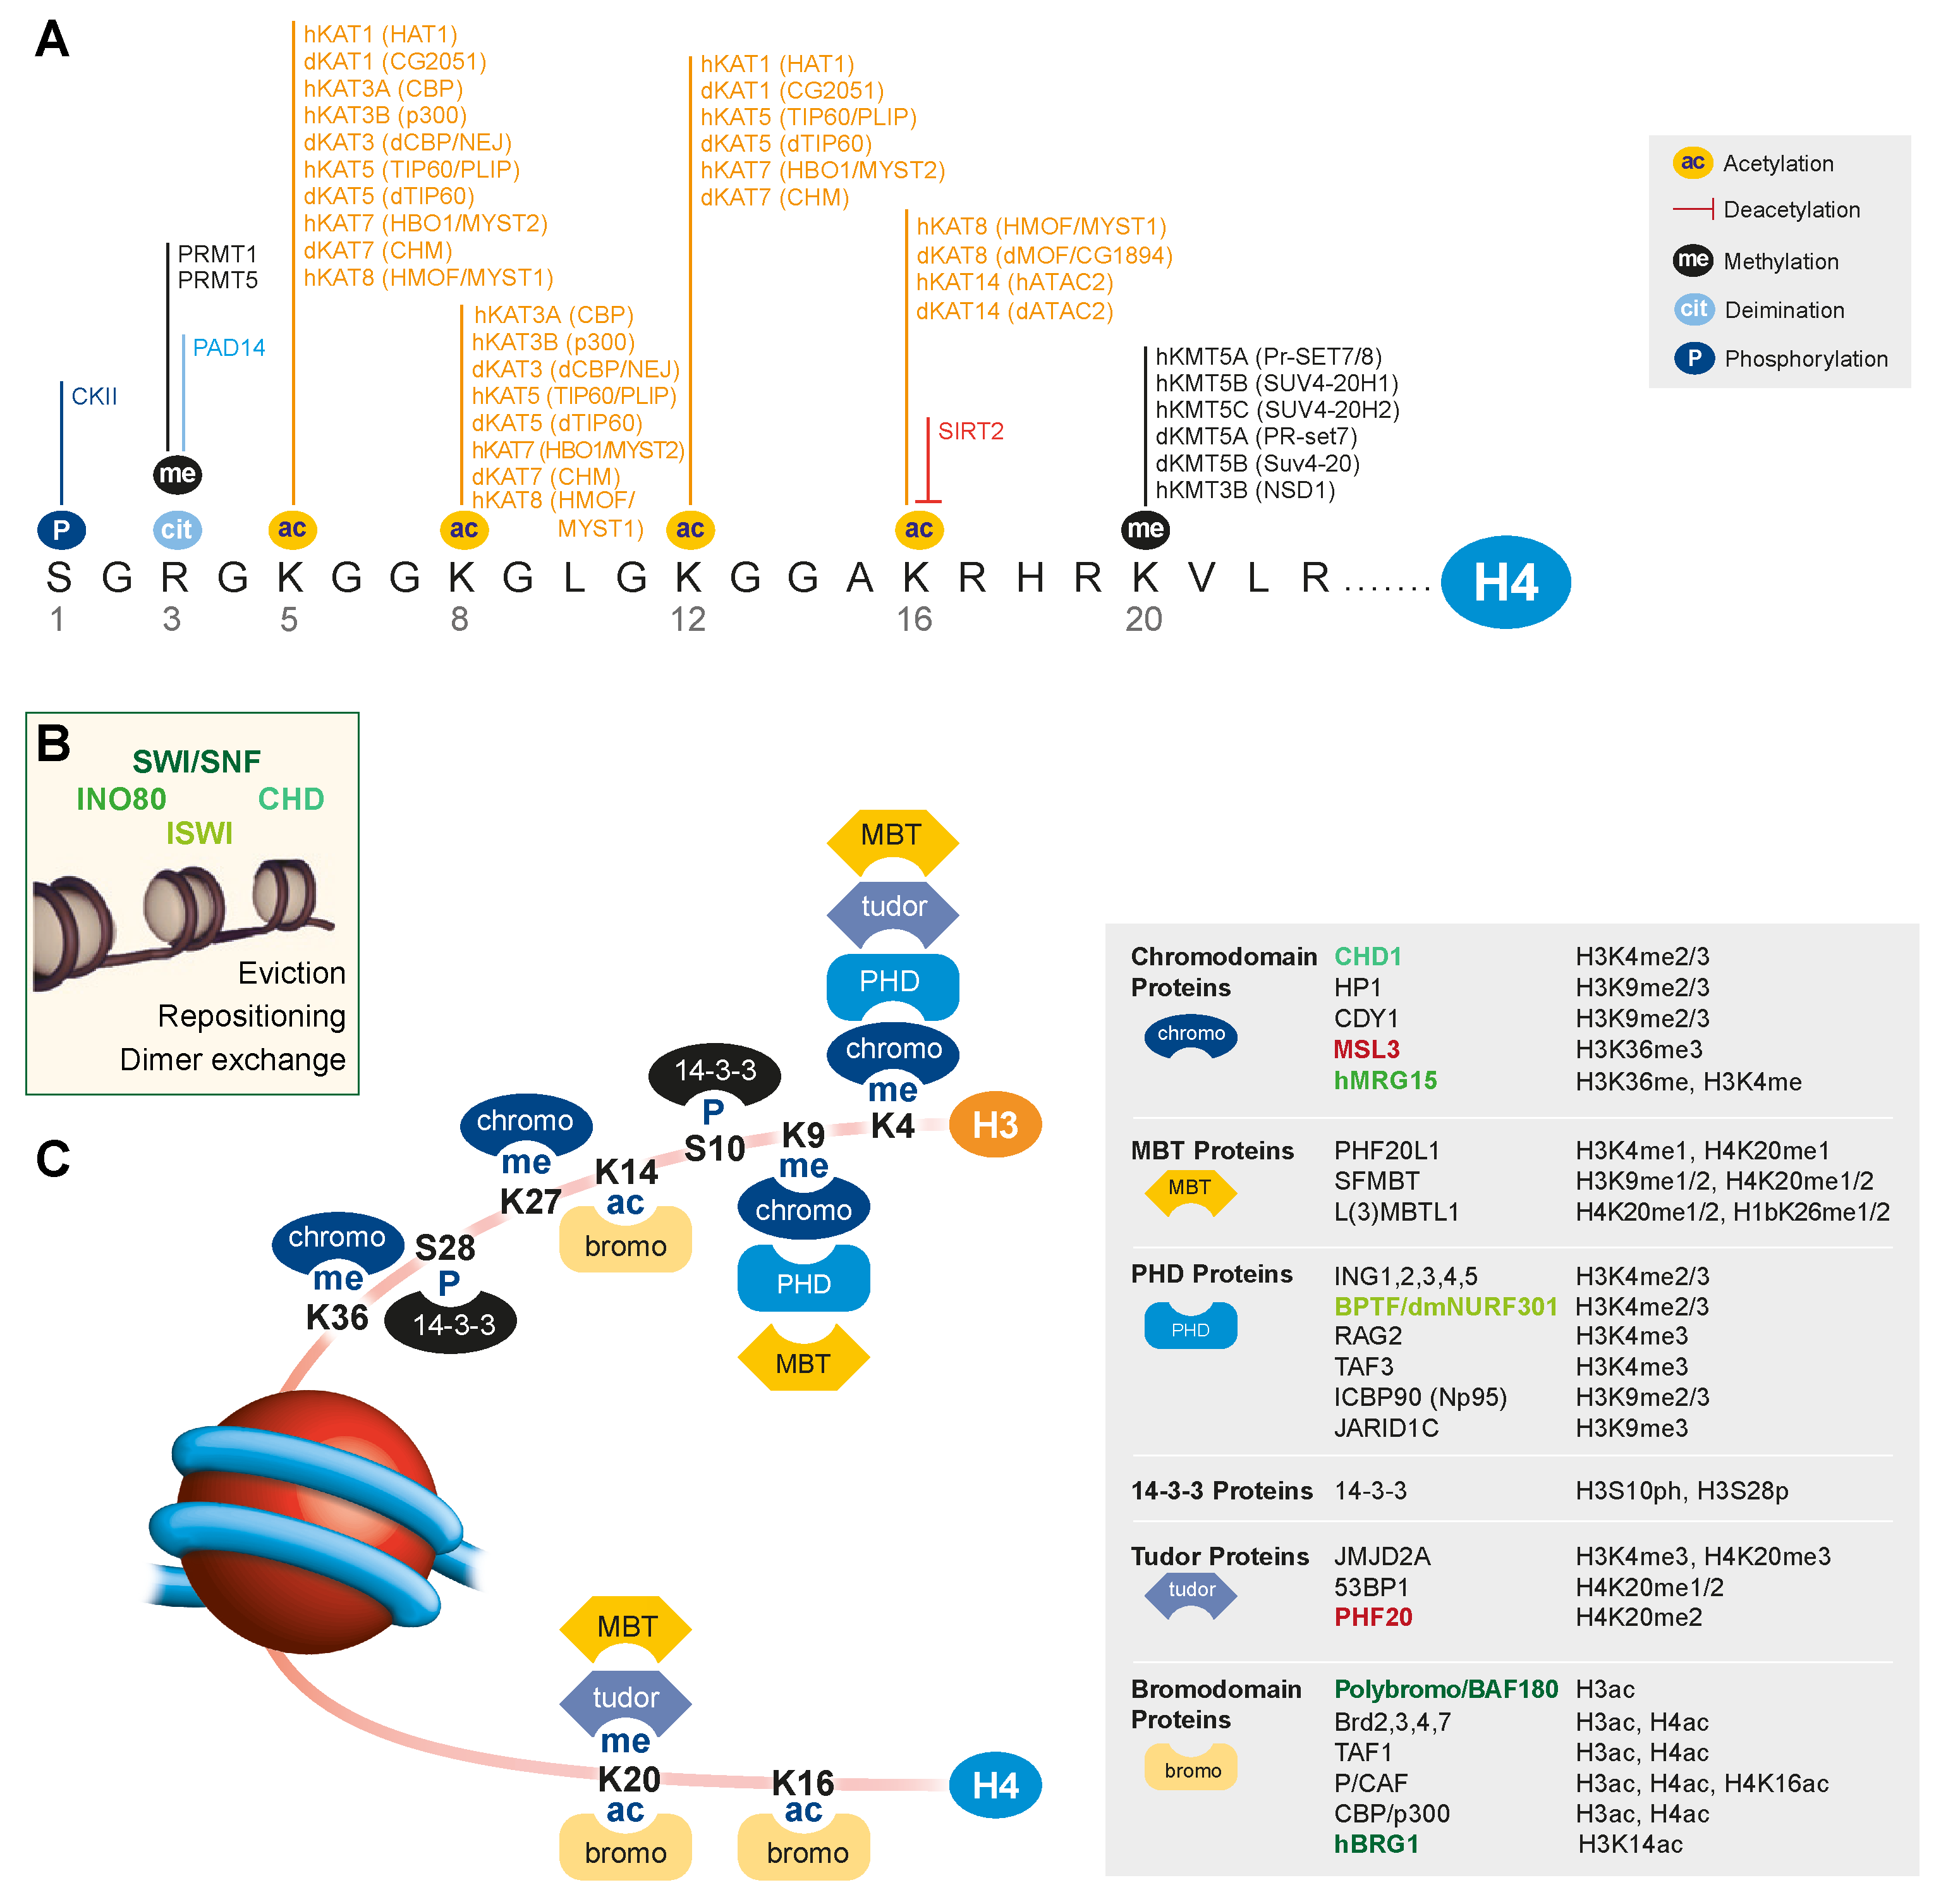
\includegraphics[width=1\textwidth]{Figures/histonesExtended.pdf}
\begin{footnotesize}
\caption[Exemplary histone modifications, their enzymes and histone-modification-recognizing protein domains.]{\textsf{Examples of histone modifications, corresponding enzymes and protein domains that recognize them.
\textbf{A)} Like for the other core histones, the tail of histone 4 (H4) contains numerous residues for covalent post-translational modifications of which some are shown here together with enzymes capable of catalyzing the respective mark in humans (h) and \textit{Drosophila} (d). Note that the different marks may have different biological meanings, e.g. methylation of H4K20 is associated with gene repression while acetylation of H4K16 is associated with gene activation (\fref{fig:histoneDistribution}). Moreover, the residues within the globular domains can also be modified (not shown). CKII = casein kinase II, PRMT = protein arginine methyltransferase, PAD2 = peptidyl arginine deiminiase, KAT = lysine acetyl transferase, KMT = lysine methyl transferase, SIRT2 = NAD-dependent deacetylase sirtuin-2. The image was taken from \citep{Abcam} and modified. See \tref{tab:HATs} for details on histone acetyl transferases.
\textbf{B)} Besides histone-modifying enzymes, chromatin remodellers greatly influence gene accessibility, too. There are four major families of ATP-dependent DNA translocases that can -- to varying degrees -- reposition, evict and replace nucleosomes. The INO80 family members are particularly important for DNA replication and repair as they can efficiently exchange histones while the multimeric complexes of the SWI/SNF family predominantly slide and evict nucleosomes \citep{Manelyte2013}.
\textbf{C)} Transcription factors (e.g. the transcription initiation factors TAF1 and 3), chromatin-remodelling complexes (shown in green, see B) and histone-modifying enzymes (e.g. the HATs CDY, p300 and P/CAF and the lysine demethylases JARID1C and JMJD2A) often contain domains that recognize specific histone modifications. Members of MOF-associated complexes are shown in red. The image was taken from \citep{Abcam} and modified.
}}
\label{fig:histonesExtended}
\end{footnotesize}
\end{figure}
%------------------------------------


%
The epigenetic influence on gene expression is based on two main properties of chromatin: its physical structure and the potential for myriad post-translational modifications of the histone residues of their N-terminal tails and globular domains (\fref{fig:histone}). The physical properties of nucleosomes can be altered by chromatin remodellers that apply a torsional strain to the DNA strand that generates enough force to change the position of a nucleosome \citep{Manelyte2013}. These ATP-dependent enzymes are required for the maintenance of active as well as silenced genome regions, they can replace the canonical core histones shown in \fref{fig:histone} with histone variants and they are required for the assembly of chromatin during DNA replication and DNA repair (reviewed by \citet{Manelyte2013}, see \fref{fig:histonesExtended} for the four families of chromatin remodellers).

Numerous histone-modifying enzymes are now known; they catalyze the transfer of small organic groups (e.g. methyl, acetyl and phosphate groups) or small proteins (e.g. ubiquitin) to histone residues, especially to their tail regions (\fref{fig:histonesExtended}). The tail domains of the histones are not essential for nucleosome formation, but their modifications contribute to the recruitment of chromatin- and DNA-binding proteins \citep{Turner2014} (see \fref{fig:histonesExtended} for histone binding domains) and serve as landmarks of active transcription (euchromatin) as well as silenced regions (heterochromatin). Although more than 100 histone modifications have been described \citep{Kouzarides2007, Tan2011} and well-defined histone mark combinations are the basis for distinct chromatin states associated with different levels of transcription \citep{Ernst2010,Kharchenko2011}  (see \fref{fig:histoneDistribution}), the debate about whether they are cause, consequence or merely a by-product of gene transcription is on-going \citep{Henikoff2011, Ptashne2013, Whitehouse2013}. On the other hand, the impact of chromatin structure on transcription is well established on at least two levels: high nucleosome density interferes with transcription factor binding and gene activation (reviewed by \citet{Henikoff2011}) and higher order chromatin domains separate euchromatin from heterochromatin, presumably to enable efficient transcription and constrain transcriptional inactivation \citep{Dixon2012}. Proteins that modify histones (e.g. methyl transferases, acetyl transferases) and ATP-dependent nucleosome remodellers have accordingly risen as a new class of transcription-related factors that do not necessarily need to directly interact with DNA to influence gene expression (\fref{fig:histonesExtended}).\\
%\begin{minipage}{\textwidth} % to avoid pagebreaks despite longtable environment
%\setlength{\extrarowheight}{2pt}
%\renewcommand{\arraystretch}{1.5}
\vspace*{-2em}
%\begin{longtable}[l]{>{\textsf\bgroup}p{3cm}<{\egroup} >{\textsf\bgroup}p{2.5cm}<{\egroup}>{\textsf\bgroup}p{5cm}<{\egroup}} % defining the columns - these must match the widths defined for the mini pages down below!
\begin{table}[t]
\begin{singlespacing}
\begin{small}
\begin{sffamily}
\caption[The main histone acetyl transferase families.]{\textsf{The main histone acetyl transferase families. The lysine acetyl transferase (KAT) designation indicates the standardized nomenclature suggested for HATs. GNAT = Gcn5-related \textsl{N}-acetyl transferase, MYST = MOZ, Ybf2/Sas3, Sas2, Tip60. The table was taken from \citet{Berndsen2008}}} %\\ % the \\ is important!
\label{tab:HATs}
\begin{tabular}{>{\small\textsf\bgroup}p{3.5cm}<{\egroup} >{\small\textsf\bgroup}p{3.5cm}<{\egroup} >{\small\textsf\bgroup}p{5cm}<{\egroup} }
%%%%%%%%%%%%%%%
% table title
\textbf{Enzyme} & \textbf{KAT designation} & \textbf{Histone specificity}
\tabularnewline \toprule
%-----------------------
\textbf{GNAT family} & & \\
Gcn5 & 2 & H3K9, 14, 36 \\
p/CAF & 2B & H3K14
\tabularnewline \midrule
%--------------------------
\textbf{MYST family} & & \\
Tip60 & 5 & H4K5, K8, K12 (K16) \\
MOF 	&	8	&	H4K5, K8, K16 \\
Sas3	&	6	&	H3K14, K23 \\
MOZ		&	6A & H3K14
\tabularnewline \midrule
%--------------------------
\textbf{p300 and others} & & \\
CBP & 3A & H2AK5, H2B \\
p300 	&	3B	&	H2AK5, H2B \\
Rtt109	&	11 & H3K56, K9, K23	
%--------------------------
\tabularnewline \bottomrule
%-----------------------------
\end{tabular}
%\label{tab:HATs}
%\end{longtable}
\end{sffamily}
\end{small}
\end{singlespacing}
\end{table}
%\end{minipage}

%===================================================================
%	SECTION 
%===================================================================
\section{The histone acetylase MOF}
The histone acetylase (HAT) MOF (males absent on the first) was discovered in a screen for an X-chromosomal factor with essential male-specific function in \textit{Drosophila melano\-gaster} \citep{Hilfiker1997}. HATs catalyze the addition of acetyl groups to histone and non-histone protein residues. Based on the catalytic subunits that show distinct structural features, HATs can be classified into three main families: GCN5-related \textsl{N}-acetyl transferases (GNATs) that typically contain bromodomains, the MYST family including MOF that is characterized by chromodomains and an additional group of less conserved proteins with HAT activity (\tref{tab:HATs}). All HATs strongly depend on the interaction with other proteins to carry out their enzymatic activity in an efficient manner \citep{Lee2007}. MOF was originally thought to function predominantly within the male-specific lethal (MSL) complex, more recent studies identified additional interaction partners with essential, sex-independent functions (non-specific lethal (NSL) proteins, see \fref{fig:MOFcomplexes}). Members of both complexes are well conserved in mammals, but particularly MOF has attracted considerable biomedical research interest as global loss of H4K16ac was identified as a hallmark of numerous cancers with corresponding misregulation of MOF \citep{Fraga2005,Pfister2008} (see \tref{tab:cancer}). Deletion of \textit{Mof} in mice leads to embryonic lethality with profound alterations of the nuclear architecture and DNA damage responses \citep{Thomas2008,Gupta2008} and mammalian MOF has been described in a variety of cellular contexts, ranging from spermatogenesis to the protection from myocardial hypertrophy in models of heart stress (\fref{fig:MYST}). The underlying mechanisms of these diverse functions have remained largely uncharacterized, but in regard to its role in gene regulation and DNA repair, significant insights have been gained, particularly in the context of its interaction partners (\fref{fig:functions}, \tref{tab:functions1}, \tref{tab:functions2}).
%--------------------------------------
%%% Figure other functions of MOF 
\begin{figure}[b]
 \begin{minipage}[c]{0.48\textwidth}
   \includegraphics[width=\textwidth]{Figures/MOFothers.png}
 \end{minipage}\hfill
 \begin{minipage}[c]{0.48\textwidth}
	\begin{footnotesize}
   \caption[Functions of the mammalian orthologue of MOF, MYST1.]{\textsf{The mammalian orthologue of \textit{Drosophila} MOF, MYST1, was shown to be required for longevity of Purkinje cells \citep{Kumar2011} and the suppression of hepatitis virus C (HCV) infections \citep{Fusco2013}. It also regulates autophagy \citep{Fullgrabe2013}, protects stressed heart cells from hypertrophy \citep{Qiao2014} and its depletion from the hypothalamus leads to diet-induced obesity \citep{Brenachot2014}. Additionally, its action is needed for the replacement of histones by protamines during spermatogenesis \citep{Meistrich1992,Thomas2007,Lu2010} and MYST1 depletion blocks T cell development \citep{Gupta2013}. Conversely, MYST1 was recently implied in maintaining ESC pluripotency \citep{Li2012}.
}}
\label{fig:MYST}
\end{footnotesize}
 \end{minipage}
\end{figure}
%---------------------------------
%------------------------------
%%% Figure MOF complexes
\begin{figure}
\includegraphics[width=1\textwidth]{Figures/MOFcomplexes.png}
\begin{footnotesize}
\caption[Protein domains and interactions of the MSL and NSL complexes.]{\textsf{Protein domains and interactions of the MSL and NSL complexes.
\textbf{A)} MOF contains a chromo-barrel domain that can bind DNA and RNA and is essential for histone acetylation \citep{Conrad2012}. The zinc finger (Zn) motif within the catalytic HAT domain interacts with MSL1, MSL3 and NSL1 \citep{Morales2004,Kadlec2011}.
\textbf{B)} MSL complex members: The PEHE domain is specific for MSL1-like proteins \citep{Marin2003}. The RING finger domain of MSL2 is required for ubiquitylation and protein-protein interactions \citep{Copps1998,Kruse2009}. MSL3's MRG domain is necessary for the targeting of the male X \citep{Buscaino2003} and preferably binds methylated lysine residues \citep{Moore2010} (\fref{fig:histonesExtended}). MLE contains N-terminal and C-terminal helicase domains with RNA and DNA remodelling activity \citep{Lee1997}.
\textbf{C)} MSL1 is a largely unstructured scaffold protein that dimerizes with MSL2 and subsequently brings together MSL3 and MOF that both interact with MSL1's PEHE domain \citep{Scott2000,Kadlec2011}. \textit{roX} RNA is bound by MSL2 and MLE, completing the complex \citep{Ilik2013}.
\textbf{D)} NSL complex members: NSL1 resembles MSL1, but lacks the region C-terminally of PEHE for the interaction with MSL3 \citep{Smith2005}; instead, like NSL2, it contains an additional WDS-interacting motif (WIN and EIDV, respectively) \citep{Dias2014}. MBD-R2 contains multiple chromatin and nucleic acid interaction motifs; the forkhead-associated domain (FHA) of MCRS2 was shown to bind phosphorylated protein residues and was identified as part of the INO80 complex \citep{}. WDS is a small scaffold protein made up of seven WD40 repeats that is also part of the histone methyl transferase MLL/SET complex \citep{Trievel2009}. 
\textbf{E)} Analogous to the MOF-MSL1 interaction, MOF is recruited into the NSL complex via an interaction with the C-terminal PEHE domain of NSL1 that also interacts with MCRS2, MBD-R2 and WDS \citep{Kadlec2011, Raja2010, Dias2014}. WDS directly interacts with NSL1 and NSL2 \citep{Dias2014}. 
All images are based on figures and data from \citep{Mendjan2006,Kadlec2011,Raja2010,Hallacli2012,Dias2014}.
}}
\label{fig:MOFcomplexes}
\end{footnotesize}
\end{figure}
%----------------------------------------
%
\subsection{The male-specific lethal (MSL) complex and dosage compensation in \textit{Drosophila}}
%
The first known MOF partners were part of the MSL complex which has been well studied in \textit{D. melano\-gaster} where its deletion leads to male-specific lethality.
Like mammals, male and female fruit flies differ in respect to the number of X chromosomes. In contrast to mammals where the inactivation of one of the two female X chromosomes extends the problem of X monosomy to both sexes \citep{Wright2012}, \textit{D.~melano\-gaster} has evolved a chromosome-wide transcriptional upregulation of the single male X chromosome (shown first in 1965 by \citet{Mukherjee1965}) that equalizes the doses of X-linked and autosomal genes in the heterogametic sex. Owing to its male-specific effects on viability and an extraordinary enrichment along the male fly X chromosome, the MSL complex was proposed as they key component of dosage compensation within \textit{Sophophora} species \citep{Ruiz2000} (reviewed by \citet{Laverty2010}).

The exact molecular mechanisms of MSL’s X-specific targeting are not completely elucidated up to date, but many details about the assembly of the complex are now known (see \fref{fig:MOFcomplexes}). The MSL complex is a ribonucleoprotein complex composed of five proteins (MOF, MSL1, MSL2, MSL3 (male-specific lethal 1-3), MLE (maleless)) and one long non-coding RNA (roX1 or roX2 (RNA on X), see \fref{fig:MOFcomplexes} for details and \tref{tab:Names} for synonyms and mammalian protein names). In flies with X:A ratios of one, SXL (sex lethal) inhibits the translation of MSL2 by recruiting the RNA-binding protein UNR (upstream of neuroblastoma rat sarcoma) to the 3’-untranslated region (UTR) of the \textit{msl2} transcript \citep{Abaza2006, Duncan2006, Hennig2014}. Lack of MSL2 suffices to inhibit the formation of the MSL complex in females although all other MSL proteins can in principle be transcribed and translated in both sexes \citep{Gorman1995, Bhadra1999}. While the recognition of the X chromosome is achieved by the MSL1/MSL2 heterodimer \citep{Lyman1997, Kadlec2011}, accumulation along the chromosome and transcription stimulation depend on the presence of \textit{all} MSL proteins (reviewed by \citet{Conrad2011}).

Within the MSL complex, the HAT enzyme MOF has been regarded as the key effector molecule for dosage compensation as the approximately twofold upregulation of X-linked genes in male \textit{Drosophila} seems linked to the long-known hyperacetylation of the male X chromosome \cite{Turner1992,Bone1994}. It was shown that MOF has an extraordinary preference to acetylate lysine 16 of histone H4 (H4K16ac) if accompanied by the MSL complex \citep{Akhtar2000, Smith2000, Li2009, Cai2010} which is in stark contrast to the rather promiscuous acetylation of various histone residues by other known HATs \citep{Lee2007} (\tref{tab:HATs}). The MSL complex, in turn, is responsible for excessive MOF recruitment to the male X chromosome and the subsequent enrichment of H4K16ac along gene bodies \citep{Turner1992, Gelbart2009} that is both stimulated and fine-tuned by the interaction of MOF with MSL complex members \citep{Morales2004, Prestel2010, Kadlec2011}.

Since the MSL complex is absent in female flies, it is unlikely that its presence is required for initial activation of X-linked gene transcription; it is instead thought to recognize already expressed genes that are localized on the X chromosome. The current model delineates that the MSL complex is recruited to several high-affinity binding sites on the X chromosome from where it spreads to active genes (i.a. aided by the binding of MSL3 to methylated H3K36, an abundant mark of on-going transcription \citep{Larschan2007} (\fref{fig:histoneDistribution})) and subsequently enhances the basal transcription rates by acetylation of H4K16 \citep{Conrad2011}. 
%
\subsection{The effects of H4K16ac on chromatin structure}
Acetylation of H3 and H4 tails in general is associated with increased chromatin accessibility as the negative charges of the acetyl group interfere with tight packaging of the poly-anionic DNA strand. In contrast to the acetylation of lysines 5, 8, and 12 of histone H4 that seem to affect the chromatin structure and transcription in a non-specific, cumulative manner, H4K16ac conveys more specific transcriptional effects \citep{Dion2005}. One explanation for H4K16’s special function is its key role in anchoring neighboring nucleosomes where unmodified H4K16 is required for the formation of strong salt bridges between the H4 tail and the acidic patch on the next histone octamer (reviewed by \citet{Kalashnikova2013, Preez2013}). Acetylation of H4K16 disrupts these salt bridges and inhibits chromatin compaction which is in line with the inhibition of chromatin fiber formation that was reported for H4K16ac specifically \citep{Shogren-Knaak2006, Robinson2008}.
%
\subsection{The effects of H4K16ac on transcription}
With the exception of yeast, H4K16ac has unanimously been associated with active transcription as open chromatin in general is a key determinant of gene expression (\citet{Lee2007, Henikoff2011}). In the context of the MSL complex and \textit{Drosophila} dosage compensation, three possible entry points for gene expression enhancement by massive H4K16ac have been proposed: 
\begin{itemize}
\item \textbf{Transcription initiation:} The high accessibility of promoter regions and regulatory elements allows transcription factors to find their cognate target sites more efficiently \citep{Chen2014} and might increase the probability of pre-initiation complex assembly \citep{Conrad2012b}, thereby elevating local concentrations of regulatory proteins and the transcription machinery itself.
\item \textbf{Pol~II pause release:} In mammals, H4K16ac was shown to recruit Brd4 (\fref{fig:histonesExtended}) which in turn recruits P-TEFb, an essential factor for the transition of promoter-bound Pol~II into its actively processing state \citep{Zippo2009} (\fref{fig:Expression}). H4K16ac might thus serve as an additional binding site for transcription-related proteins.
\item \textbf{Elongation of transcription:} Based on the observation that H4K16ac generally covers the entire gene body of dosage-compensated genes with increasing signals towards the 3’-end, it has been suggested that the main effects of H4K16ac for dosage compensation should be on transcription elongation \citep{Smith2001}. This is supported by a recent study reporting Pol~II to reach the 3’-end of genes more easily on the X chromosome compared to autosomes which was dependent on the presence of MSL2 \citep{Larschan2011}. 
\end{itemize}
%---------------------------------------
%%% Figure MOF-complexes-associated functions
\begin{figure}[b!]
\includegraphics[width=1\textwidth]{Figures/Functions.png}
\begin{footnotesize}
\caption[Molecular functions of MOF and its interaction partners in transcription activation and cell-cycle-related processes.]{\textsf{The vast majority of functions associated with MOF and its interaction partners are related to general transcriptional activation and the cell cycle. Displayed here are those functions that have either been reported to involve MOF within the context of the NSL and MSL complex or individual complex members. Not shown are the roles of WDR5 (WDS) and MCRS1 (MCRS2) as part of the methyl lysine transferase MLL/SET complex and the nucleosome remodelling INO80 complex, respectively.
Grey lines indicate that proteins were found to physically interact, colored arrows indicate post-translational modifications by either MOF (acetylation (ac)) or MSL2 (ubiquitylation (ub)). The details of the function are summarized in \tref{tab:functions1} and \tref{tab:functions2}.
}}
\label{fig:functions}
\end{footnotesize}
\end{figure}
%------------------------------------
The fact that H4K16ac stimulates transcription, perhaps via different mechanisms, is not contested \citep{Birchler2003, Conrad2011}. However, how the approximately twofold upregulation of male single copy X-linked genes to the levels of autosomal genes \citep{Hamada2005, Straub2005} is achieved, has not been solved yet. Given the multiple chromatin, protein, DNA and RNA interaction as well as catalytic domains present in the MSL complex (\fref{fig:MOFcomplexes}, \tref{tab:enzymes}), it is likely that its effects on transcription are manifold and reach beyond H4K16ac to ensure the modest, but vitally important transcription enhancement of male X-linked genes.\\
\begin{minipage}{\textwidth}
\setlength{\abovecaptionskip}{-2ex}
\setlength{\belowcaptionskip}{-2ex}
\vspace*{-2em}
%\begin{landscape}
\begin{minipage}{\textwidth}
\begin{singlespacing}
\begin{small}
\begin{sffamily}
\begin{longtable}[l]{>{\textsf\bgroup}p{3.8cm}<{\egroup} >{\raggedright\arraybackslash}p{2.7cm} >{\textsf\bgroup}p{7cm}<{\egroup}}
\caption[MOF-associated proteins in transcription activation.]{\textsf{MOF-associated proteins in transcription activation. Related to \fref{fig:functions}.}} \\ % the \\ is important! see http://tex.stackexchange.com/questions/103698/extra-alignment-tab-with-longtable
%%%%%%%%%%%%%%%
% table title
\textbf{Proteins} & \textbf{Function} & \textbf{Biological effect}
\tabularnewline \toprule
%\endfirsthead % indicates that the lines above appear as head of the table on the first page
%\multicolumn{3}{c}%
%{\tablename\ \thetable\ -- \textit{Continued from previous page}} \\ [2ex]
%\textbf{Proteins} & \textbf{Function} & \textbf{Biological effect}
%\tabularnewline \toprule \tabularnewline [1ex]
%\endhead % Line(s) to appear at top of every page (except first)
%\multicolumn{3}{r}{\textit{Continued on next page}} \\
%\endfoot % Last line(s) to appear at the bottom of every page (except last)
%\endlastfoot
%%%%%%%%%%%%%%%%%%%
%%% let's start the table content; each column (often) gets its own minipage which enables itemized lists etc.
%%%%%%%%%%%%%%%%%%%
%% first row
%-----------------------
%\\ \multicolumn{3}{c}{\textbf{\textsf{Gene expression}}}
%\\ [2ex] \hline \\ [1ex]
%------------------
\begin{minipage}[c]{3.8cm}
				\vskip 2pt
					MOF within the\\MSL complex \\
				(MSL1, MSL2,\\MSL3, MLE (roX))
				\vskip 2pt
			\end{minipage}
			& \begin{minipage}[c]{2.7cm}
					\raggedright acetylation of H4K16ac \citep{Akhtar2000,Taipale2005,Li2009} \\
			\end{minipage}
					& \begin{minipage}[c]{7cm}
					\vskip 2pt
									\begin{itemize}[noitemsep, leftmargin=*]
										\item opening of chromatin (reviewed by \citet{Preez2013})
										\item dosage compensation in male \textit{D.~melano\-gaster} that entails the upregulation of the entire X chromosome \citep{Conrad2011}
									\end{itemize}				
									\vskip 2pt
							\end{minipage}
%\\ [2ex] \hline \\ [1ex]
\tabularnewline \midrule
%-----------------------
\begin{minipage}[c]{3.8cm}
\vskip 2pt
					MOF within the\\NSL complex \\
				(NSL1, NSL2, NSL3,\\MCRS2, MBD-R2, WDS)
				\vskip 4pt
			\end{minipage}
			& \begin{minipage}[c]{2.7cm}
							\raggedright acetylation of H4K16 \citep{Li2009}, H4K5, H4K8 \citep{Cai2010}
			\end{minipage}
					& \begin{minipage}[c]{7cm} % 3rd column
									\begin{itemize}[noitemsep, leftmargin=*]
										\item opening of chromatin \citep{Preez2013}
										\item housekeeping gene regulation \citep{Feller2012, Lam2012}
									\end{itemize}				
							\end{minipage}
%\\ [2ex] \hline \\ [1ex]
\tabularnewline \midrule
%-----------------------
\begin{minipage}[c]{3.8cm}
					MSL2
			\end{minipage}
			& \begin{minipage}[c]{2.7cm}
			\vskip 2pt
					\raggedright ubiquitylation of H2BK34 \citep{Wu2011}
					\vskip 4pt
			\end{minipage}
					& \begin{minipage}[c]{7cm} % 3rd column
					\vskip 2pt
							implicated to stimulate methylation of H3K4 \citep{Wu2011} and transcription elongation \citep{Wu2014}
							\vskip 4pt
							\end{minipage}
\tabularnewline \midrule
%\\ [2ex] \hline \\ [1ex]
%-----------------------
\begin{minipage}[c]{3.8cm}
\vskip 2pt
					MCRS2
					\vskip 4pt
\end{minipage}
			& \begin{minipage}[c]{2.7cm}
			\vskip 2pt
					interaction partner
					\vskip 4pt
			\end{minipage}
					& \begin{minipage}[c]{7cm} % 3rd column
					\vskip 2pt
							facilitates Pol~II recruitment to target genes \citep{Andersen2010}
							\vskip 4pt
						\end{minipage}
%\\ [2ex] \hline\pagebreak
%-----------------------
%\multicolumn{3}{c}{\textbf{\textsf{Cell-cycle-associated processes}}}
%\\ [2ex] \hline \\ [1ex]
%-----------------------
%%%%%%%%%%%%%%%%%%%%%%%%%%
\tabularnewline \bottomrule
\label{tab:functions1}
\end{longtable}
\end{sffamily}
\end{small}
\end{singlespacing}
\end{minipage}

%\vspace*{-2em}
\begin{minipage}{\textwidth}
\begin{singlespacing}
\begin{small}
\begin{sffamily}
\begin{longtable}[l]{>{\raggedright\arraybackslash}p{3cm} >{\raggedright\arraybackslash}p{11cm}}
\caption[MOF-associated proteins in cell-cycle-related processes.]{\textsf{MOF-associated proteins in cell-cycle-related processes. Related to \fref{fig:functions}}} \\ % the \\ is important! 
%%%%%%%%%%%%%%%
% table title
\textbf{Biological process} & \textbf{Observation} 
\tabularnewline \toprule
%==========================
\begin{minipage}[c]{3cm}
					G2/M checkpoint
			\end{minipage}
					& \begin{minipage}[c]{11cm} % 3rd column
					\vskip 4pt
							NSL1, NSL2, NSL3, MCRS2, MBD-R2 and WDS were identified as essential factors for G2/M checkpoint progression following DNA damage in \textit{D.~melano\-gaster} \citep{Kondo2011}
							\vskip 4pt
							\end{minipage}
\tabularnewline \midrule
%\\ [2ex] \hline \\ [1ex]
%-----------------------
\begin{minipage}[c]{3cm}
					mitotic spindle
			\end{minipage}
					& \begin{minipage}[c]{11cm} % 3rd column
					\vskip 4pt
							\begin{itemize}[noitemsep, leftmargin=*]
							\item NSL2 is needed for mitotic spindle assembly \citep{Goshima2007}
							\item MCRS1 stabilizes the mitotic spindle \citep{Meunier2011}
							\item WDS was identified in a screen for microtubule-associated proteins \cite{Hughes2008}
							\end{itemize}
							\vskip 2pt
							\end{minipage}
\tabularnewline \midrule
%------------------------
\begin{minipage}[c]{3cm}
					apoptosis
			\end{minipage}
					& \begin{minipage}[c]{11cm} % 3rd column
					\vskip 4pt
							\begin{itemize}[noitemsep, leftmargin=*]
							\item ubiquitylation of p53 by MSL2 leads to accumulation of p53 in the cytoplasm \citep{Kruse2009} which is necessary for apoptosis \cite{Muscolini2011}
							\item MOF acetylates p53 in the presence of NSL1 \citep{Li2009} which is necessary for apoptosis induction in cells with DNA damages \citep{Sykes2006, Sykes2009}
							\item human MBD-R2 (PHF20) stimulates expression of p53 and prevents its degradation via a direct interaction with methylated p53 \citep{Park2009, Cui2012}
							\end{itemize}
							\vskip 2pt
							\end{minipage}
\tabularnewline \midrule
%------------------------
\begin{minipage}[c]{3cm}
					DNA repair
			\end{minipage}
					& \begin{minipage}[c]{11cm} % 3rd column
					\vskip 4pt
							\begin{itemize}[noitemsep, leftmargin=*]
								\item MOF is generally required for repair of DNA double strand breaks and recruitment of 53BP1 and BRCA \cite{Sharma2010, Li2010}; its phosphorylated form is particularly important for biasing the cells towards homologous repair during S~phase by displacing 53BP1 from the site of the DNA damage \citep{Gupta2014}
								\item human MSL2 ubiquitylates 53BP1 \citep{Lai2013}
								\item human MSL1 interacts with 53BP1 that positively stimulates DNA damage repair \citep{Gironella2009}
							\end{itemize}
							\vskip 2pt
							\end{minipage}
%%%%%%%%%%%%%%%%%%%%%%%%%%
\tabularnewline \bottomrule
\label{tab:functions2}
\end{longtable}
\end{sffamily}
\end{small}
\end{singlespacing}
\end{minipage}
\end{minipage}
%
\subsection{Individual functions of MSL1 and MSL2}
Evidence for activities of the individual MSL complex members besides MOF predominantly stems from studies on the mammalian orthologues that exist in a sex-independent manner without apparent preference for a particular chromosome (\tref{tab:functions1} and \ref{tab:functions2}). While this seems to strip the MSL complex in mammals of its exceptional and highly visible role for dosage compensation, it also opens up a large scope of putative chromatin-related functions that might not depend on MOF. The ubiquitylation of lysine 34 of histone 2B (H2BK34ub) by MSL2, for example, is stimulated by the presence of MSL1, but not MOF \citep{Wu2011}. Moreover, MSL1 and MSL2 were reported to directly interact with P-TEFb, thereby aiding the transition of Pol~II to elongation \citep{Wu2014} (see \fref{fig:Expression}).

In addition to direct effects on transcription-related processes, MSL1 and MSL2 have been implied in DNA repair and apoptosis, primarily due to their interaction with the tumor suppressor p53 and the p53-binding protein (53BP1) \citep{Kruse2009, Li2010, Lai2013} (see \fref{fig:functions} and \tref{tab:functions2} for details). These tasks do not necessarily exclude the possibility for MOF interactions as histone acetylation and general chromatin relaxation seem to stimulate the DNA repair pathways \citep{Altmeyer2013}, but these findings indicate that, like MOF, MSL proteins might also act outside the MSL complex context, especially in non-sophophora species.
%
\subsection{The non-specific lethal complex and additional MOF targets}
Using mass spectrometry, \citet{Mendjan2006} identified additional, sex-unspecific interaction partners of MOF in fly and human cell cultures which were termed non-specific lethal (NSL) proteins owing to the fact that mutations in their genes killed flies of both sexes.

The NSL complex is comprised of seven proteins: MOF, NSL1, NSL2, NSL3 (non-specific lethal 1-3), MCRS2 (microspherule protein), MBD-R2 (methyl-binding domain protein), and WDS (will die slowly; see \tref{tab:Names} for synonyms and mammalian protein names). At the beginning of my PhD studies, little was known about the cellular task conveyed by the NSL complex, but the first genome-wide study by \citet{Raja2010} had laid the foundation for establishing the NSL complex as a ubiquitous interaction partner that could explain the MSL-independent binding that had been observed for MOF on male as well as female autosomes \citep{Bhadra1999, Kind2008, Raja2010}. Complementary, biochemical experiments revealed that the interaction with NSL proteins relaxes MOF’s substrate specificity towards additional histone residues (H4K5, H4K8) \citep{Cai2010}. Furthermore, MOF was reported to be capable of acetylating non-histone targets which predominantly entail proteins that guard the integrity of the genome, such as ATM (Ataxia Telangiectasia mutated), p53, DBC1 (deleted in breast cancer) and NRF2 (nuclear respiratory factor) \citep{Gupta2005, Sykes2006, Zheng2013, Chen2014}. \citet{Li2009} demonstrated that the interaction with NSL1, but not MSL1, allowed MOF to efficiently acetylate p53 which is important for the induction of apoptosis in cells suffering DNA damage \citep{Sykes2006, Sykes2009}. This finding corroborated the notion that the NSL complex might extend the impact of MOF beyond dosage compensation.
%
\subsection{Individual functions of NSL complex members}
In line with MOF’s acetylation of DNA damage response proteins, it is perhaps more than an interesting side note that all NSL complex members were shown to be essential for the G2/M checkpoint (supplemental material of \citet{Kondo2011}) and individual factors have been described in additional cell-cycle- and DNA-repair-related functions (see \fref{fig:functions}, \tref{tab:functions2}). Besides genome-wide association studies that have implicated mutations in the mammalian orthologues of \textit{Nsl1} and \textit{Nsl2} in different syndromes associated with intellectual disabilities \citep{Itsara2012, Koolen2012, Zollino2012, Gilissen2014}, NSL1-3 have remained largely uncharacterized. The mammalian counterparts of MCRS2 and WDS (MCRS1/MSP58 and WDR5, \tref{tab:Names}) have raised more research interest since they were found within additional multimeric chromatin complexes: MCRS1 was shown to interact with the chromatin remodellers INO80, NuRD and SWI/SNF \citep{Jin2005, Shimono2005, Hsu2012} (\fref{fig:histonesExtended}), while WDR5 is an essential part of the histone methyl transferase MLL \citep{Trievel2009} (mixed-lineage leukemia) that is responsible for trimethylation of H3K4, a prominent histone mark of active gene promoters (\fref{fig:histoneDistribution}). Furthermore, MCRS1 has been identified as an oncogene and a negative regulator of human telomerase reverse transcriptase (hTERT), directly suggesting a substantial influence on cellular senescence signaling \citep{Hsu2012,Hsu2014} (see \tref{tab:cancer} for cancer-related observations for the individual proteins).

As mentioned previously, most studies reporting functions of the (mammalian) NSL complex members examined the proteins in either isolated or different interaction contexts; insights into the functions of the NSL complex as an entity were lacking at the beginning of my PhD studies. One of my major aims therefore was to investigate the chromatin-associated functions of the NSL complex in \textit{Drosophila} and mouse.
%%%%%%%%%%%%%%%%%%%%%%%%%%%%%%%%%%%%%%%%%%%%%%%%%%%%%%%%%%%%%%
\section{ChIP-seq for the study of transcription factor binding}
%
The current state-of-the-art method to examine the binding profiles of DNA- and chro\-ma\-tin-in\-ter\-acting proteins \textit{in vivo} is chromatin immunoprecipitation (ChIP) followed by high-throughput NDA sequencing (seq). The endorsement of ChIP-seq as the major means to study transcription factors and histone modifications in a genome-wide fashion was made possible by the steep decline of costs for DNA sequencing during the past decade which was driven by the development of massively parallel sequencing that, in contrast to the traditional Sanger sequencing, yields rather short (35-100~bp), but highly abundant DNA reads.
%
\subsection{Chromatin immunoprecipitation}
%
%---------------------------------
%%% Figure ChIP-seq bias sources 
\begin{figure}[tb]
 \begin{minipage}[c]{0.65\textwidth}
   \includegraphics[width=\textwidth]{Figures/chip.png}
 \end{minipage}\hfill
 \begin{minipage}[c]{0.3\textwidth}
	\begin{footnotesize}
   \caption[Technical issues during ChIP-seq experiments that can interfere with the bioinformatic analysis.]{\textsf{Technical issues during ChIP-seq experiments that can interfere with the bioinformatic analysis can occur during every step of the sample preparation. The understanding of the biases introduced by the Illumina sequencing platform has increased profoundly during the past years, but the influence of the fixation and sonication procedures are much less elucidated \citep{Teytelman2013, Gavrilov2014}. See \tref{tab:biases} for details of additional biases. The upper two illustrations were taken from \citep{WikiChIP}.}}
\label{fig:ChIPseq}
\end{footnotesize}
 \end{minipage}
\end{figure}
%---------------------------------
To identify regions of the genome bound by a protein of interest (or marked by a histone modification), the protein-chromatin interactions are usually fixed with formaldehyde before the chromatin is fragmented into pieces of 200-1,000~bp. Then, an antibody against the protein of interest is used to precipitate those fragments to which the protein is bound. After de-crosslinking, the DNA can be purified and sequenced (\tref{tab:sequencing}). Numerous alterations and variations to the basic ChIP protocol exist, such as the use of micrococcal nuclease to fragment the DNA by digestion rather than sonication \citep{Kasinathan2014} and the omission of the formaldehyde fixation (native ChIP) \citep{Neill2003}. The resolution of the binding sites can be increased up to the single base level by applying an exonuclease digestion step after the ChIP (ChIP-exo) \citep{Rhee2011}. Furthermore, Nano-ChIP and linear and \textit{in vitro} transcription (LinDA) have been suggested to enable ChIP-seq with very low cell numbers \citep{Adli2011, Shanka2011}.
%
\subsection{High-throughput sequencing (Illumina platforms)}
Illumina’s high-throughput sequencing method requires short DNA fragments that are eventually hybridized to a sophisticated glass slide, the flow cell (see details in \tref{tab:sequencing}). To ensure a signal that will be unambiguously detected, each fragment is massively and clonally amplified using solid-phase PCR to generate clusters of identical molecules. The sequencing of the fragment ends (35–100~bp) itself is based on fluorophore-labelled dNTPs with reversible terminator elements that will become incorporated and excited by a laser one at a time and thereby enable the identification of single bases \citep{Illumina}. For mammalian genomes, it is recommended to sequence at least 20-60 million DNA fragments, depending on the biological question and the nature of the expected signal \citep{Chen2012, Landt2012, Jung2014}.\\
%%
%
\input{Tables/Table_Sequencing}
%
\subsection{Limitations of ChIP-seq}
Eventhough it is the method of choice for genome-wide transcription factor binding and histone mark profiling, ChIP-seq protocols are prone to biases and artifacts and must therefore be highly optimized (\fref{fig:ChIPseq}, \tref{tab:biases}). There are four factors that determine the success of a ChIP-seq experiment \citep{Liu2010, Chen2012}: the antibody (which must be rigorously tested to exclude cross-reactivity and ensure specificity and sensitivity \citep{Landt2012}), the chromatin extraction (that tends to overrepresent highly transcribed regions \citep{Waldminghaus2010, Teytelman2013}), the library preparation and sequencing (which can introduce several biases) and the bioinformatic analysis that must be tailored to match the data set’s characteristics in order to reveal biologically meaningful insights. It should be noted that all ChIP-seq experiments to date reflect the protein-DNA interactions of a population of cells which suggests that particularly strong signals represent binding sites where the protein of interest is found in the majority of cells.\\
%
\noindent\begin{minipage}{\textwidth} % to avoid pagebreaks despite longtable environment
%\begin{landscape}
\begin{singlespacing}
\begin{small}
\vspace*{-2em}
%\setlength{\abovecaptionskip}{-10pt}
\begin{longtable}{>{\textsf\bgroup\raggedleft\arraybackslash}p{3cm}<{\egroup} >{\textsf\bgroup}p{5cm}<{\egroup} >{\textsf\bgroup}p{6cm}<{\egroup}} % defining the columns - these must match the widths defined for the mini pages down below!
\caption[Biases and artifacts of ChIP-seq data.]{\textsf{Biases and artifacts of ChIP-seq data. Given a rigorously tested antibody, ChIP-seq still suffers from additional technical problems that are due to the sequencing process as well as bioinformatic hurdles.}} \\ % the \\ is important! see http://tex.stackexchange.com/questions/103698/extra-alignment-tab-with-longtable
%%%%%%%%%%%%%%%
% table title
\textbf{Problem} & \textbf{Reasons} & \textbf{Solutions}
\tabularnewline
%-----------------------
\toprule
\begin{minipage}{3cm}
				%\vskip 6pt
					\textbf{Chromatin context} and \textbf{transcription}
				%\vskip 4pt
			\end{minipage}
			&	\begin{minipage}{5cm}
				%\vskip 6pt
				\begin{itemize}[noitemsep,leftmargin=*]
					\item euchromatic chromatin is more easily fragmented
					\item formaldehyde fixation does not capture short-lived protein-DNA interactions \citep{Gavrilov2014} and pref\-er\-en\-tially cross\-links proteins with each other \citep{Neill2003}
					\item chromatin extraction may unspecifically enrich for highly active genes \citep{Teytelman2013}
				
				\end{itemize}
					%\vskip 4pt
			\end{minipage}
			& \begin{minipage}{6cm}
				\vskip 6pt
					\begin{itemize}[noitemsep,leftmargin=*]
						\item cell-type- and condition-specific input controls \citep{Vega2009, Landt2012}
						\item if possible, avoid crosslinking \citep{Neill2003, Kasinathan2014}
						\item optimized chromatin extraction including extensive de-crosslinking, RNase and Proteinase treatments \cite{Waldminghaus2010}
						\item to identify hyper-ChIPable regions, ChIP against a non-endogenous protein was suggested \citep{Teytelman2013}
						\item immunoprecipitation with immunoglobulin G (IgG, mock IP) \citep{Landt2012,Marinov2014}
						
					\end{itemize}	
				\vskip 4pt
			\end{minipage}
\tabularnewline  \hline 
%---------------------------
\begin{minipage}{3cm}
				%\vskip 6pt
					\textbf{Sequencing errors\\and errors in base calling}
				%\vskip 4pt
			\end{minipage}
			& \begin{minipage}{5cm}
				\vskip 6pt
				\begin{itemize}[noitemsep,leftmargin=*]
					\item imperfect sequencing chemistry and signal detection
					\item loss of synchronized base-incorporation into the single molecules within one cluster of clonally amplified DNA frag\-ments (phasing and pre-phasing) (see \tref{tab:sequencing})
					\item signal intensity decay
				\end{itemize}
					\vskip 4pt
			\end{minipage}
				& \begin{minipage}{6cm}
				%\vskip 6pt
					\begin{itemize}[noitemsep,leftmargin=*]
					\item improvement of the sequencing chemistry and detection
					\item optimized software for base calling \citep{Ledergerber2011}
					\item computational removal of bases with low base calling scores \citep{Minoche2011}
					\end{itemize}
				%\vskip 4pt
				\end{minipage}
\tabularnewline  \hline 
%-----------------------
\begin{minipage}{3cm}
				%\vskip 6pt
					\textbf{GC bias} and\\
					\textbf{duplicate reads}
				%\vskip 4pt
			\end{minipage}
			&	\begin{minipage}{5cm}
				%\vskip 6pt
					\begin{itemize}[noitemsep,leftmargin=*]
						\item GC-rich regions are preferably amplified by PCR
						\item small fragments are preferably hybridized to the flow cell
						\item low number of founder DNA frag\-ments
					\end{itemize}
				%\vskip 4pt
			\end{minipage}
			& \begin{minipage}{6cm}
				\vskip 6pt
					\begin{itemize}[noitemsep,leftmargin=*]
						\item optimizing cross-linking, sonication, and the ChIP protocol to ensure that the majority of the genome is present in the sample
						\item limiting PCR cycles during library preparation to a minimum
						\item computational correction for GC content \citep{Cheung2011, Benjamini2012} and elimination of reads from identical DNA fragments
					\end{itemize}	
				\vskip 4pt
			\end{minipage}
\tabularnewline  \hline 
%-----------------------------
\begin{minipage}{3cm}
				%%\vskip 6pt
					\textbf{Copy number\\variations and\\mappability}
				%\vskip 4pt
			\end{minipage}
			&
			\begin{minipage}{5cm}
				%\vskip 6pt
				\begin{itemize}[noitemsep,leftmargin=*]
					\item incomplete genome assemblies
					\item strain-specific differences to the reference assembly may lead to misrepresentation of individual loci
					\item repetitiveness of genomes and shortness of sequencing reads hinder unique read alignment
				\end{itemize}
					%\vskip 4pt
			\end{minipage}
			& \begin{minipage}{6cm}
				\vskip 6pt
					\begin{itemize}[noitemsep,leftmargin=*]
										\item increased sequencing depth and control (non-ChIP) sample aid the computational identification of problematic loci \citep{Bailey2013, Chen2012, Jung2014, Landt2012, Kidder2011}
										\item longer sequencing reads
										\item paired-end sequencing \citep{Chen2012, Bailey2013}
										\item exclusion of blacklisted regions that are known to attract artificially high read numbers \citep{Carroll2014, Blacklists}
										\item computational correction for mappability \citep{Cheung2011}
										\item considering the \textit{effective} genome size \citep{Zhang2008}
					\end{itemize}	
				\vskip 4pt
			\end{minipage}
\tabularnewline \bottomrule
%-----------------------------
\label{tab:biases}
\end{longtable}
\end{small}
\end{singlespacing}
%\end{landscape}
\end{minipage}
%
\subsection{ChIP-seq data processing}
The bioinformatic analysis of ChIP-seq data consists of numerous steps and only the very first tasks are widely standardized: The initial conversion of images of fluorescence into intensity files and ultimately text files that contain the sequencing information is typically done in an automated fashion with vendor-supplied software \citep{Ledergerber2011} (yellow boxes in \fref{fig:ChIPseq}). The resulting file contains all available information for each DNA read, such as the sequence (represented as a string of A, T, G, C), the read ID (referring to the location of the fragment cluster on the flow cell) and quality scores for every base. 
%%%%%%%%%%%%%%%%%%%%%%%%%%
\begin{figure}[tb]
 \begin{minipage}[c]{0.6\textwidth}
   \includegraphics[width=\textwidth]{Figures/DataProcessing.png}
 \end{minipage}\hfill
 \begin{minipage}[c]{0.37\textwidth}
	\begin{footnotesize}
   \caption[Overview of typical computational steps following the completion of high-throughput sequencing.]{\textsf{Overview of typical computational steps following the completion of high-throughput sequencing. The short DNA reads representing the ends of the DNA fragments hybridized onto the sequencer's flow cell are generated by the vendor-supplied software and first need to be aligned to a reference genome. Identification of significantly enriched binding sites (peak calling) and normalized coverage files are the basis for the vast majority of commonly applied ChIP-seq downstream analyses. For more details, see \tref{tab:biases} and the text. I have significantly modified and complemented the original scheme taken from \citet{Park2009}.}}
\label{fig:dataProcessing}
\end{footnotesize}
 \end{minipage}
\end{figure}
%%%%%%%%%%%%%%%%%%%%%%%%%%
Subsequent processing of the sequencing data is aggravated by the large size of the files that require powerful computational infrastructure and efficient handling and manipulation with non-mainstream software tools. UNIX-based operating systems that have traditionally been employed for scientific data analyses provide numerous commands and utilities that tend to perform very specific tasks and are commonly executed through a text-based command interpreter, the UNIX shell. In addition, various programming languages can be used either within the pipelines or for stand-alone scripts (e.g. shell scripts, awk, sed, perl, python, R). Thus, bioinformaticians constantly struggle to find a balance between highly specialized, often improvised solutions and standardized, less flexible programs while trying to ensure reproducibility and transparency through myriad rounds of iteratively adjusted analyses.
%
\subsubsection{Genome alignment}
The first task of any ChIP-seq analysis is to identify the genomic locus of origin for each DNA read. Due to the large number of reads (several millions) and the genome they originated from (almost three giga base pairs for humans), so-called mapping programs must balance accuracy, speed, computational memory usage and flexibility \citep{Leleu2010}. Various mapping algorithms exist \cite{Flicek2009}, the two most commonly used programs are bowtie2 \citep{Langmead2012} and BWA \cite{Li2010a}.

All programs offer manifold options to tune the alignment process to be either faster or more sensitive. Moreover, users can decide how to deal with ambiguous alignments (a read might match more than one region in the genome), gaps and insertions, individual base qualities within a read and mismatches \citep{Langmead2009, Langmead2012}. ChIP-seq data does not strongly depend on the exact DNA sequence of every individual DNA read because the final readout is the number of reads overlapping at particular genomic loci compared to background regions (\fref{fig:readsCoverages}), which is why mapping results are often accepted with 3-5\% of mismatched bases per read \citep{Bardet2012}. Conversely, ChIP-seq samples can suffer severely from biases that affect the distribution of background reads across the genome which must be assessed and ultimately accounted for \citep{Liu2010, Cheung2011, Benjamini2012} (see \tref{tab:biases}). 
%%%%%%%%%%%%%%%%%%%%%%%%%%%%%%%%%%
\begin{figure}[tb]
 \begin{minipage}[c]{0.6\textwidth}
   \includegraphics[width=\textwidth]{Figures/CoverageAndReads.png}
 \end{minipage}\hfill
 \begin{minipage}[c]{0.37\textwidth}
	\begin{footnotesize}
   \caption[Snapshot of a typical visualization of DNA read and coverage files.]{\textsf{Snapshot of a typical visualization of DNA read and coverage files. Shown here are paired-end reads, i.e. both ends of each DNA frag\-ment were sequenced (indicated by dark and light blue boxes) and can now be used to easily reconstruct the precise frag\-ments. The coverage shown on top is based on the number of overlapping fragments.}}
\label{fig:readsCoverages}
\end{footnotesize}
 \end{minipage}
\end{figure}
%%%%%%%%%%%%%%%%%%%%%%%%%%%%
\subsubsection{Control sample}
Some biases associated with ChIP-seq data are caused by the genome structure, the chromatin context as well as bioinformatic processing that vitally depends on the state of the genome annotation (\tref{tab:biases}). These systematic errors are generally thought to be controlled by the use of a matching input sample \citep{Kharchenko2008b, Zhang2008, Park2009, Kidder2011, Ho2011, Chen2012, Landt2012}, i.e. a sample that underwent the same treatment as the ChIP-seq sample (in regard to the cell culture, fixation, lysis, fragmentation (\fref{fig:ChIPseq})) with the exception of the immunoprecipitation step. It is recommended to generate a control for every chromatin preparation, for each cell type and condition and to sequence the control at least as deeply as (or preferably deeper than) the ChIP sample \citep{Tuteja2009,Ho2011,Landt2012, Bailey2013}. The goal of the input sample is to have a comprehensive representation of the background reads that should allow the assessment of under- and overrepresented regions due to biological factors (e.g. heterochromatic regions) \citep{Vega2009} as well as technical reasons (e.g. unmappable regions and Ultra High Signal regions \citep{Blacklists}).

To account for biases introduced by the chromatin precipitation (\fref{fig:ChIPseq}, \tref{tab:biases}), some researchers prefer to perform a mock immunoprecipitation (IP) with a non-specific immunoglobulin instead of an input sample \citep{Landt2012}. Unfortunately, the DNA recovery of mock IP experiments can be exceedingly small which could lead to overrepresentation of sequencing artifacts (\tref{tab:biases}). Moreover, it was shown that the use of histone H3 or H4 ChIP-seq does not significantly improve the analysis of ChIP-seq data for histone marks compared to the above mentioned input \citep{Flensburg2014}.
%
\subsubsection{Quality controls and metrics}
%
In the past two years, several measures for the assessment of ChIP-seq data quality have been proposed, most notably by the ENCODE (encyclopedia of DNA elements) consortium that generated hundreds of now publicly available ChIP-seq data sets \citep{Consortium2012}. The quality checks are applied at all stages of the data processing, starting with the determination of contaminant sequences in the raw read files, followed by the quantification of uniquely and non-redundant reads after read alignment and possible overrepresentation of GC-rich regions (\tref{tab:biases}). Reads with more than one optimal alignment locus in the genome are usually filtered out in most ChIP-seq analyses as they might increase the risk of false positive binding site detections. However, if the protein of interest is expected to be enriched at repetitive regions of the genome, it would be detrimental to eliminate these ambiguous reads that usually originate from repeats \citep{Treangen2012}. See \tref{tab:qscores} for the summary of the most widely used quality metrics including those that assess the reproducibility since two replicates per ChIP-seq and input samples are recommended \citep{Rozowsky2009, Landt2012}.

Once the basic sequencing quality properties are checked, scores for signal-to-noise ratios should give an impression of how well the ChIP worked. It is important to note that the vast majority of the quality controls were optimized for ChIP-seq data of transcription factors and histone marks with abundant and very localized enrichments. ChIP-seq experiments with broad, domain-like enrichments or very few binding sites will very often not meet the recommended quality thresholds due to their inherently reduced signal-to-noise ratios \citep{bamFingerprint, Landt2012, Bailey2013, Diaz2012} (\tref{tab:qscores}). 
%
\subsubsection{Normalized fragment coverages}
One part of the ChIP-seq analysis workflow that is often mentioned, but rarely scrutinized in detail is the generation of coverage files for which the read-focused information from the genome alignment is converted into integer counts of the number of reads at a given genomic locus (\fref{fig:dataProcessing}, \fref{fig:readsCoverages}). This conversion serves two purposes: a)~the possibility to adjust for coverage biases and b)~file size reduction which is essential for efficient downstream analysis tools, data sharing and visualization. The aim of the normalization is to make different samples comparable, irrespective of their sequencing depth and additional biases. 

Despite its importance, there is no agreement on the optimal generation of coverage files (except for extending the reads to match the expected original DNA fragment size \citep{Pepke2009, Leleu2010}, \fref{fig:readsCoverages}). Numerous strategies for the normalization of differing numbers of total reads per sample exist (e.g. linear scaling factors calculated with various methods \citep{Kharchenko2008b, Rozowsky2009, Diaz2012}, reads per million per kilobase \citep{Mortazavi2008}, quantile normalization \citep{Mendoza2012}, trimmed mean of M-values \citep{Robinson2010}) and two methods for the correction of GC bias have been presented \citep{Cheung2011, Benjamini2012}.
%
\subsubsection{Identification of binding sites}
In addition to coverage files, downstream analyses of ChIP-seq data are usually based on a set of genome regions that represent loci where the immunoprecipitated protein had bound \citep{Park2009,Liu2010, Bailey2013}. These regions should be overrepresented in the ChIP-seq sample compared to the genome-wide background (hence they are commonly referred to as peaks) and numerous algorithms have been developed to separate binding events from background noise (reviewed by \citet{Pepke2009}). The two basic steps of peak calling are: 1.~identification of regions with large numbers of overlapping reads and 2.~the assessment of the significance of the read enrichment.
The programs choose slightly different approaches for both steps, influencing the sensitivity, specificity, but most strongly the positional accuracy of the peak region predictions \citep{Wilbanks2010}. The reliability of the significance measures absolutely depends on the choice of the statistical model to describe the distribution of background reads which is complicated by the numerous sources of coverage bias mentioned previously and in \tref{tab:biases}. 

One of the most widely used tools, MACS \citep{Zhang2008}, tries to accommodate for the sample-specific influences of the experimental as well as the bioinformatic procedures by utilizing dynamic Poisson distributions. They are parametrized on the background reads of each sample to capture the genome-wide values as well as local biases surrounding any candidate region taking the input control into consideration. To account for false positive calls, MACS version 1.4 calculates an empirical false discovery rate based on significantly enriched regions in the input sample \citep{Zhang2008, Feng2012}. 

Peak calling can be tremendously helpful for ChIP-seq analyses, but thorough benchmarking of the performance of the different algorithms is severely hindered by the lack of a comprehensive list of true binding sites that could be used for a fair comparison. In addition to ChIP-qPCR validation of selected peak regions \citep{Laajala2009}, several proxies for peak quality have been used, such as DNA motif enrichments \citep{Wilbanks2010} and reproducibility between different peak calling algorithms \citep{Laajala2009}. None of these approaches offer a global verification of peak regions, particularly not in regard to their exact position. Therefore, manual inspection is still the method of choice to decide on the success or failure of a peak calling step \citep{Rye2011}. This is especially important when dealing with diffuse, domain-like signals for which great inconsistencies between different peak callers were reported \citep{Ho2011}. 
%
\subsubsection{Downstream analyses}
Exploratory ChIP-seq analyses strongly depend on visualization and unsupervised clustering of the data to unveil unexpected patterns and correlations that can subsequently be experimentally tested \citep{Ramirez2014}. There is virtually no standardization regarding downstream analyses as they must be tailored to the specific biological questions, but the most widely applied strategies are depicted in \fref{fig:dataProcessing}. For example, \textit{de novo} identification of DNA motifs underlying the ChIP-seq peaks is helpful to understand the targeting of a transcription factor \citep{Machanick2011} and gene ontology terms of putative target genes may give clues to the biological role of the investigated protein \citep{Huang2009, Welch2014} (see \tref{tab:tools} for commonly used programs). Furthermore, additional genome-wide data sets are often integrated to complement the ChIP-seq; transcriptomics, for example, can be used to directly correlate the binding of a protein to transcriptional regulation of possible target genes \citep{Chelmicki2014}.
%
\section{Aims}
% Chapter Template

%\chapter{Aims} % Main chapter title

%\label{Aims} % for referencing this chapter elsewhere, use \ref{ChapterX}

%\lhead{Aims} % this is for the header on each page - perhaps a shortened title

%------------------------------------------------------------------
%	SECTION 
The goal of my studies was to gain biological insights from the analyses of the binding profiles of MOF-associated proteins: the non-specific lethal complex (NSL) and the male-specific lethal complex (MSL) members.
The analyses were based on chromatin immunoprecipitation followed by high-throughput sequencing (ChIP-seq). Thus, before the biological questions could be addressed, we first needed to establish robust bioinformatic workflows and scripts ranging from data processing to bias identification and correction and manifold customized downstream analyses. 

In \textit{Drosophila}, we specifically wanted to address whether the different complex members of the NSL complex would co-occur. Moreover, we wanted to infer and subsequently test new hypotheses about the biological function of the NSL complex in regard to gene expression regulation.
Since both MSL and NSL complex had not been previously examined in mammals, we then set out to study their chromatin targeting in mouse cells. To this end, Tomasz Chelmicki generated ChIP-seq profiles of MOF, MSL1, MSL2, NSL3 and MCRS1 in mouse embryonic stem cells and neuronal progenitor cells. The ChIP-seq data study revealed common and different binding principles of the two complexes in pluripotent and differentiated cells which we complemented with transcriptome studies from perturbation experiments and additional genome-wide data sets.




